\documentclass[tikz,border=2pt]{standalone}
\usepackage{amsmath,amssymb}
\usepackage{tikz}
\usetikzlibrary{arrows.meta}

\begin{document}
% Setup cost K is paid once per order regardless of its size: small batches mean many setups
% (rate KD/y large), large batches spread one K over more units.
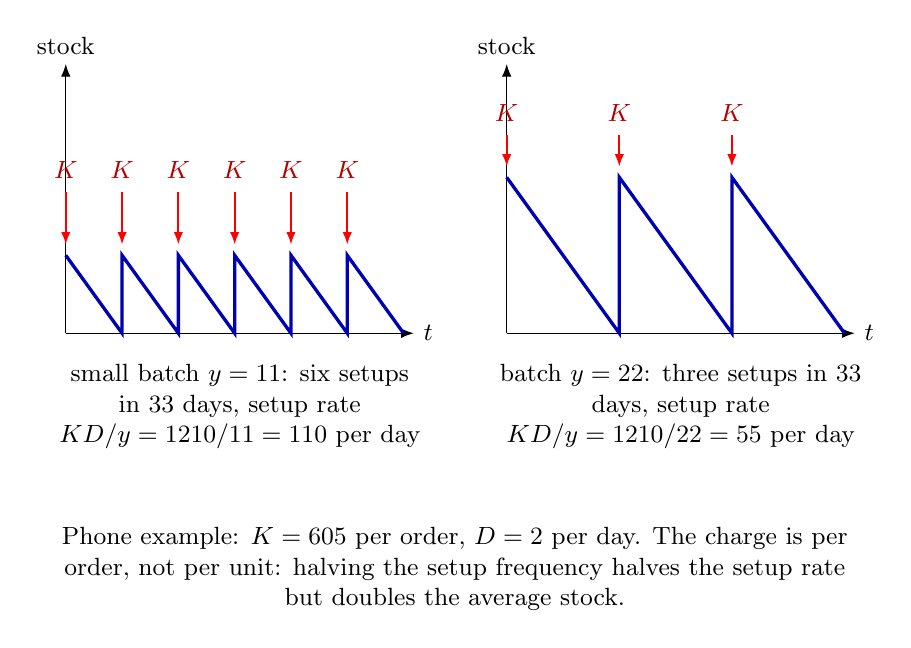
\begin{tikzpicture}[every node/.style={font=\small}, >={Latex[length=1.6mm]}, x=0.13cm, y=0.09cm]
	\begin{scope}
		\draw[->] (0,0) -- (34,0) node[right] {$t$};
		\draw[->] (0,0) -- (0,38) node[above] {stock};
		\draw[blue!70!black, very thick] (0,11) -- (5.5,0) -- (5.5,11) -- (11,0) -- (11,11) -- (16.5,0) -- (16.5,11) -- (22,0) -- (22,11) -- (27.5,0) -- (27.5,11) -- (33,0);
		\foreach \t in {0,5.5,11,16.5,22,27.5} {\draw[->, red, thick] (\t,20) -- (\t,12.5); \node[red!70!black, anchor=south] at (\t,20.5) {$K$};}
		\node[anchor=north, align=flush center, text width=4.6cm] at (17,-3) {small batch $y=11$: six setups in $33$ days, setup rate $KD/y=1210/11=110$ per day};
	\end{scope}
	\begin{scope}[xshift=5.6cm]
		\draw[->] (0,0) -- (34,0) node[right] {$t$};
		\draw[->] (0,0) -- (0,38) node[above] {stock};
		\draw[blue!70!black, very thick] (0,22) -- (11,0) -- (11,22) -- (22,0) -- (22,22) -- (33,0);
		\foreach \t in {0,11,22} {\draw[->, red, thick] (\t,28) -- (\t,23.5); \node[red!70!black, anchor=south] at (\t,28.5) {$K$};}
		\node[anchor=north, align=flush center, text width=4.6cm] at (17,-3) {batch $y=22$: three setups in $33$ days, setup rate $KD/y=1210/22=55$ per day};
	\end{scope}
	\node[anchor=north, align=flush center, text width=10cm] at (38,-26) {Phone example: $K=605$ per order, $D=2$ per day. The charge is per order, not per unit: halving the setup frequency halves the setup rate but doubles the average stock.};
\end{tikzpicture}
\end{document}
